\chapter{Partial Coloring Methods}\label{ch:partial}

The linear algebraic method from Chapter~\ref{ch:linalg} is a powerful
tool for taking advantage of the structure of a set system when
proving discrepancy upper bounds. We saw that it can be used to give significantly improved
discrepancy upper bounds 
over those 
achieved by random colorings for many natural set systems, e.g.,
set systems of bounded degree, and set systems induced by rectangles
or by permutations. 

However, it is not at all clear how to use this method to match, let alone improve the upper bound $\disc(\SS)
\lesssim \sqrt{n \log(2n)}$ for a set system $\SS$ of $O(n)$ subsets of a
universe of $n$ elements, achieved by a random coloring.
In this
chapter, we develop the method of partial colorings, which combines the
power of randomization with the ability of the linear algebraic method
to take advantage of weak dependencies between sets in a set
system. 
We give a number of applications of the method, including a
proof of Spencer's Six Standard Deviations Suffice Theorem showing the discrepancy upper bound
above can be improved to $\disc(\SS) \lesssim \sqrt{n}$.

\section{Beck's Partial Coloring Lemma}

To build some intuition for partial coloring methods, we start with
the simplest of them: the partial coloring lemma of Beck. 

A general
theme of discrepancy upper bounds is decomposing a set system into
a potentially large number of small sets, and a small number of
potentially large sets. We saw this in the proof of the Beck-Fiala
theorem in Chapter~\ref{ch:linalg}, where we showed that a set system
\(\SS\) of maximum degree \(\ssdeg(\SS)\) on a universe of size \(n\)
has at most \(\frac{n}{c}\) sets of size greater than
\(c\ssdeg(\SS)\). This is useful, since it is easier to control the
discrepancy of small sets, and when the large sets are not too many,
keeping their discrepancy low imposes a small number of constraints on
our colorings. In Chapter~\ref{ch:linalg} we used linear algebra to
formalize this intuition. Beck's lemma below gives another
formalization, based on a beautiful combination of combinatorial and
probabilistic reasoning.

In preparation, we prove a simple combinatorial lemma, showing that in
any large enough set of colorings, at least two colorings must
disagree on many elements. Stronger statements are known, but we state
one with an elementary proof, as it suffices for our needs.

\begin{lemma}\label{lm:ch3-hamming}
  Suppose \(\mathcal{C} \subseteq \{-1,+1\}^n\) is a set of colorings
  of size \(|\mathcal{C}| \ge 2^{n/2}\). Then there exist two colorings
  \(\col,\col' \in \mathcal{C}\) such that
  \[
    |\{i: \col(i) \neq \col'(i)\}| \ge n/10.
  \]
\end{lemma}
\begin{proof}
  Let us fix any $\col \in \mathcal{C}$. The
  number of colorings \(\col'\in \{-1,+1\}^n\) for which \(|\{i
  : \col(i) \neq \col'(i)\}| \le n/10\) is
  \[
    \sum_{i = 0}^{\lfloor n/10\rfloor} {n \choose i}
    \le
    2^{n H(1/10)} < 2^{n/2} \le |\mathcal{C}|.
  \]
  where \(H(p) \eqdef -p \log_2 p - (1-p)\log_2(1-p)\) is the binary
  entropy function, and we used standard estimates on the volumes of
  Hamming balls (e.g.~Proposition 3.3.3 in~\cite{guruswami2012essential}).
  Then there must be at least one $\col' \in \mathcal{C}$
  for which $|\{i: \col(i) \neq \col'(i)\}| \ge
  n/10$.
\end{proof}

We are now ready to prove Beck's partial coloring lemma. The lemma applies to set systems $\SS$ partitioned into a set system $\SS_1$, typically consisting of the large sets, which should be relatively few, and a set system $\SS_2$, typically consisting of the small sets. The lemma guarantees that one can find a partial coloring (\ie, a coloring that's allowed to assign color $0$ to a constant fraction of elements), which has discrepancy $0$ on sets in $\SS_1$, and has discrepancy matching the one achieved by a random coloring on $\SS_2$.

\begin{lemma}\label{lm:ch3-beck}
  Let $\SS_1$ and $\SS_2$ be set systems on a set $\uni$ of size $n
  \ge 3$
  such that  $|S| \le s$ for all $S \in \SS_2$, and
  \[
  \prod_{S \in \SS_1}{(2|S| + 1)} \le 2^{(n-1)/5}.
  \]
  Then there exists a {partial coloring} $\col:\uni \to \{-1, 0, +1\}$
  such that
  \begin{enumerate}
  \item $\col(S) = 0$ for all $S\in \SS_1$;
  \item $|\col(S)| \lesssim \sqrt{s \log(2|\SS_2|)}$ for
    all $S \in \SS_2$;
  \item \(|\{\elem \in \uni: \col(\elem) \neq 0\}| \ge n/10.\)
  \end{enumerate}
  \end{lemma}
\begin{proof}
  Let $\col'$ be chosen uniformly at random from $\{-1, +1\}^\uni$. By the union bound and Hoeffding's inequality,
  \[
    \Pr\left[\max_{S \in \SS_2} |\col'(S)| > t \right]
    \le 2|\SS_2| e^{-t^2/2s}.
  \]
  When \(t \eqdef \sqrt{2s \ln(4|\SS_2|)},\) this is at most $1/2$, and therefore the set
  \[
    \mathcal{C} \eqdef \left\{\col'\in \{-1,+1\}^\uni : \disc(\SS_2,\col')\le \sqrt{2s \ln(4|\SS_2|)}\right\}
  \]
%  $\mathcal{C}$ of colorings
 % $\col'$ of $\uni$ with discrepancy $\disc(\SS_2,\col') \le \sqrt{2s \ln(4|\SS_2|)}$
  has size $|\mathcal{C}| \ge 2^{n-1}$. 

  On the other hand, the number of different values that the vector
  $(\col'(S))_{S \in \SS_1}$ can take as \(\col'\) ranges over
  \(\{-1,+1\}^\uni\) is at most $\prod_{S \in
    \SS_1}{(2|S| + 1)}$, which is bounded by $2^{(n-1)/5}$ by
  assumption. 
  By the pigeonhole
  principle, there must be a set $\mathcal{C}' \subseteq \mathcal{C}$
  of colorings of $\uni$ of size  $|\mathcal{C}'| \ge
|\mathcal{C}|/2^{(n-1)/5} \ge 2^{4(n-1)/5}$ such that any two
  $\col', \col'' \in \mathcal{C}'$ satisfy $\col'(S) = \col''(S)$ for
  all $S\in \SS_1$. As \(4(n-1)/5 \ge n/2\) for \(n
  \ge 3\), applying Lemma~\ref{lm:ch3-hamming} to \(\mathcal{C}'\)
  shows that there exist two colorings \(\col',\col''\in
  \mathcal{C}'\) that differ on at least
  \(n/10\) elements of \(\uni\). 
  We can now take $\col \eqdef \frac12(\col' - \col'')$ as our
  partial coloring. As \(\col(\elem) \in \{-1,1\} \) whenever \(\col'(\elem)
  \neq \col''(\elem)\), \(\col\) colors properly at least
  \(n/10\) elements of \(\uni\), proving the third property of \(\col\). The
  first property holds because \(\col'(S) = \col''(S)\) for all \(S
  \in \SS_1\), so \(\col(S) = \frac12(\col'(S) - \col''(S)) = 0\). The
  second property holds since \(\col',\col''\in \mathcal{C}\), so for
  any \(S \in \SS_2\) we have
  \[
    |\col(S)| \le \frac12(|\col'(S)| + |\col''(S)|) \le \sqrt{2s \ln(4|\SS_2|)}. \qedhere
  \]
 % This proves the lemma.
\end{proof}


Note that the proof of
Lemma~\ref{lm:ch3-beck}, unlike the linear algebraic arguments in
Chapter~\ref{ch:linalg}, does not suggest an efficient algorithm to
find the partial coloring. The main issue is the use of the pigeonhole
argument on the exponentially large set of colorings \(\mathcal{C}\)
to construct $\mathcal{C}'$.

Lemma~\ref{lm:ch3-beck} is a refinement of the discrepancy bounds we can
get from a uniformly random coloring. In particular, if $\SS_1$ is
empty, then we can, with high probability, achieve the same
discrepancy on $\SS_2$ as in the lemma with a full uniformly random
coloring. Being able to set the discrepancy of some sets to $0$,
however, allows us to prove discrepancy bounds that are not achieved
by a random coloring (except with exponentially small probability). As an illustration, we
prove a bound for the Beck-Fiala problem. Later in the chapter
we will see more advanced techniques that allow proving sharper
bounds. 

\begin{theorem}\label{thm:ch3-bf-weak}
  For any set system \((\SS, \uni)\) with maximum degree
  \(\ssdeg(\SS)\) and \(|\uni| = n > 1\), 
  we have \(\disc(\SS) \lesssim \sqrt{\ssdeg(\SS)} \log(n)^{2}\). 
\end{theorem}
\begin{proof}
  Let us assume that \(n \ge 3\), as otherwise the theorem is
  trivially true. Similarly, we can assume
  that \(\ssdeg(\SS) \le n^2\), since the trivial upper
  bound of \(\disc(\SS) \le n\) holds for any coloring.
  As in the proof of Lemma~\ref{lm:ch2-bf-counting}, 
  the number of sets in \(\SS\) satisfies \(|\SS| \leq n\ssdeg(\SS) \le
  n^3\). 
  
  We define \(\SS_1 \eqdef \{\set \in \SS: |\set| > s\}\) and
  \(\SS_2 \eqdef \{\set \in \SS: |\set| \le s\}\) for a parameter
  \(s\) that we choose later. By Lemma~\ref{lm:ch2-bf-counting},
  \(
  |\SS_1| < n\ssdeg(\SS)/s,
  \)
  and, therefore,
  \[
    \prod_{\set \in \SS_1}{(2|\set| + 1)} \le (2n+1)^{n\ssdeg(\SS)/s}
    = 2^{n\log_2(2n+1)\ssdeg(\SS)/s}.
  \]
  In order to apply Lemma~\ref{lm:ch3-beck}, we need that the exponent
  on the right is at most \((n-1)/5\), so we set
  \(
  s \eqdef C\log_2(2n+1) \ssdeg(\SS),
  \)
  for a sufficiently large constant $C>0$.
  Then the lemma gives us a partial coloring \(\col:\uni \to \{-1, 0,
  +1\}\) with discrepancy
  \[
    \disc(\SS, \col) \lesssim  \sqrt{\ssdeg(\SS)\log_2(n) \log(2|\SS_2|)}
    \lesssim  \sqrt{\ssdeg(\SS)} \log(2n),
  \]
   where we used the trivial
  bound \(|\SS_2| \le |\SS| \le  n^3\). Moreover,
  Lemma~\ref{lm:ch3-beck} guarantees that the set \(\act \eqdef
  \{\elem \in \uni: \col(\elem) = 0\}\) satisfies \(|\act|
  \le 9n/10\).

  To obtain a full coloring, we can iterate this process. In
  particular, as $\ssdeg(\SS|_\act) \le \ssdeg(\SS)$, we can
  inductively
  find a coloring \(\col'\) of the restriction \(\SS|_\act\), and assign the color in $\col'$ to the elements that are given color $0$ by $\col$. As there are $O(\log n)$ iterations, the overall discrepancy can increase by a factor at most $O(\log n)$, giving the bound $O(\sqrt{\ssdeg(\SS)}\log(n)^2)$, as desired. 
  %of the set system
  %to the currently uncolored elements. We then assign the color of any
  %element \(\elem \in \uni \setminus \act\) according to \(\col\), and
  %the color of any element \(\elem \in \act\) according to \(\col'\). 
  % The overall discrepancy is then bounded by
  % \[
  %   \disc(\SS) \lesssim \sqrt{\ssdeg(\SS)} \sum_{k = 0}^{\lfloor
  %     \log_{10}n\rfloor} \log(2n 0.9^{k})^{1.5}
  %   \lesssim \sqrt{\ssdeg(\SS)}\log(2n)^{2.5}. \qedhere.
  % \]
\end{proof}

\section{A Stronger Partial Coloring Lemma, and Applications}

While Beck's partial coloring lemma is a powerful tool, it often gives
suboptimal bounds with large poly-logarithmic factors, as we saw in
the case of the Beck-Fiala problem. Intuitively, one reason for this
is that the lemma only allows setting two types of discrepancy bounds
for the partial coloring: a set either receives \(0\) discrepancy, or
the discrepancy it would get under a random coloring. More precise
bounds can be derived by allowing more freedom in setting discrepancy
bounds. In this section, we state a stronger partial coloring lemma
that follows this approach, and present some applications of it. We
prove the lemma later in the chapter, as a corollary of a more general
geometric result.

\subsection{Statement}

Next we state this stronger partial coloring lemma. Rather than
restrict ourselves to set systems, we adopt a more general linear
algebraic formalism. The proof of Lemma~\ref{lm:ch3-partial} is deferred to Section~\ref{sec:ch3-giann}.

\begin{lemma}\label{lm:ch3-partial}
  Let \(v_1, \ldots, v_m \in \R^n\) be such that \(\|v_i\|_2 \le 1\)
  for each \(i\), and let \(\lambda_1, \ldots, \lambda_m\) be
  positive reals. For any \(s > 0\), define the function
  \begin{equation}\label{eq:ch3-partial}
    \parcol(s) :=  \begin{cases}
      1.5\exp(-s^2/8) & s\ge 4\\
      \ln\left(20/s^2\right) & s < {4}
    \end{cases}.
  \end{equation}
  If \(\sum_{i=1}^m \parcol(\lambda_i) \le n/8\), then there exists a partial coloring
  \(\col \in \{-1,0,+1\}^n\) such that, for all \(i \in [m]\),
  \(|\ip{v_i,\col}| \le \lambda_i\|v_i\|_2\), and \(|\{j: \col(j) \neq 0\}|
  \ge n/10\). 
\end{lemma}

To apply Lemma~\ref{lm:ch3-partial} to a set system
$\SS \eqdef \{S_1, \ldots, S_m\}$, we can choose each $v_i$ to be the indicator vector of the set $S_i$, and, if we want the bound $|\col(S_i)| \le d_i$,
we can set $\lambda_i \eqdef d_i/\sqrt{|S_i|}$.

We can now compare
Lemmas~\ref{lm:ch3-beck}~and~\ref{lm:ch3-partial}. Suppose that
$\SS_1 = \{S_1, \ldots S_k\}$, and $\SS_2 = \{S_{k+1}, \ldots, S_m\}$,
where any set in $\SS_2$ has size at most $s$, and define
$v_1, \ldots, v_m$ as above. If we set
$\lambda_i = 1/\sqrt{2|S_i|}$ for $i \in [k]$, and
$\lambda_i = \sqrt{8\ln(12|\SS_2|)}$ for each $i \in \{k+1, \ldots, m\}$, then a partial
coloring $\col$ such that $|\ip{v_i,\col}| \le \lambda_i$ for all
$i \in [m]$ would satisfy $|\col(S)| < 1$, and thus
$\col(S) = 0$ for $S \in \SS_1$, and also
$|\col(S)| \lesssim \sqrt{s \log(2|\SS_2|)}$ for $S \in \SS_2$, as
in Lemma~\ref{lm:ch3-beck}. Lemma~\ref{lm:ch3-partial} guarantees such
a coloring if
\[
  \sum_{S \in \SS_1} \ln(40|S_i|) \le (n-1)/8.
\]
For comparison, the requirement in Lemma~\ref{lm:ch3-beck}
can be re-written as
\[
  \sum_{S \in \SS_1} \log_2(2|S| + 1) \le (n-1)/5,
\]
which is of the same form. Thus,  Lemma~\ref{lm:ch3-partial} allows us
to recover an analogous statement to
Lemma~\ref{lm:ch3-beck}. However, Lemma~\ref{lm:ch3-partial}  gives
us much more freedom in setting the $\lambda_i$ parameters. We
illustrate how this freedom translates to better discrepancy bounds
with the next two applications.

\subsection{Applications}

%We illustrate the power of Lemma~\ref{lm:ch3-partial} with two
%applications: a proof of Spencer's Six Standard Deviations Suffice
%Theorem, and an improved bound for the Beck-Fiala problem.

\paragraph{Spencer's Theorem.}
For our first application we consider an arbitrary set system
\((\SS, \uni)\) of \(m \eqdef |\SS|\) sets on a universe of size \(n
\eqdef |\uni|\). Recall that a random coloring achieves a discrepancy
of \(O(\sqrt{n \log m})\), and, in the absence of additional structure,
it is reasonable to conjecture that this is tight. Surprisingly, this
is not the case, and a celebrated result of Spencer shows that, for
any \(m \ge n\),
\(\disc(\SS) \lesssim \sqrt{n \log(2m/n)}\). In particular, when $m=O(n)$, we get a discrepancy bound of \(O(\sqrt{n})\),
showing that the logarithmic term incurred by a random coloring is
unnecessary. In fact, Spencer showed that when \(m = n\) the
discrepancy is at most \(6\sqrt{n}\), and his result is often
referred to as the Six Standard Deviations Suffice theorem.
% Spencer's proof was a sophisticated version of the proof of Beck's
% partial coloring lemma (Lemma~\ref{lm:ch3-beck}). Here we present a
% different, geometric approach to the theorem, due to Gluskin and Giannopoulos.

Using Lemma~\ref{lm:ch3-partial}, we prove the following slightly stronger statement for matrices with bounded entries.
\begin{theorem}\label{thm:ch3-spencer}
  For any \(m \times n\) matrix \(\mat \in [-1, +1]^{m\times n}\),
  where $m \ge n$, we have
  \(\disc(\mat) \lesssim \sqrt{n\log(2m/n)}\). %In particular, for any
  %set system \((\SS, \uni)\) consisting of \(m\) sets on a universe of
%  size \(n\), \(\disc(\SS) \lesssim \sqrt{n\log(2m/n)}\).
\end{theorem}
%The second claim in Theorem~\ref{thm:ch3-spencer} 
Spencer's result follows with $M$ as the incidence matrix of \(\SS\).

The core of the proof of Theorem~\ref{thm:ch3-spencer} is the
following partial coloring result.
\begin{lemma}\label{lm:ch3-spencer-partial}
For any \(m \times n\) matrix \(\mat \in [-1, +1]^{m\times n}\),
  where $m \ge n$, there exists a partial coloring
  \(\col \in \{-1,0,+1\}^n\) such that
  \(\|\mat \col\|_\infty \lesssim \sqrt{n\log(2m/n)}\) and
  \(|\{i: \col(i) \neq 0\}| \ge n/10\).
\end{lemma}
\begin{proof}
  We use Lemma~\ref{lm:ch3-partial}, where vector $v_i$ is the $i$-th
  row of $\mat$, and
  \(
  \lambda_i \eqdef \sqrt{8\ln(12m/n)}.
  \)
  Then the statement follows from Lemma~\ref{lm:ch3-partial}.
\end{proof}

%Similarly to the proof of Theorem~\ref{thm:ch3-bf-weak}, 
We can show
Theorem~\ref{thm:ch3-spencer} by iteratively applying
Lemma~\ref{lm:ch3-spencer-partial}  to obtain
a full coloring. The key observation in the case of Spencer's theorem
is that the discrepancy of partial colorings decreases rapidly
with \(n\) and thus the discrepancy of the full coloring only increases by a constant factor.

\begin{proof}[Proof of Theorem~\ref{thm:ch3-spencer}]
  Let \(\col\) be as in Lemma~\ref{lm:ch3-spencer-partial}
  Then the set \(\act \eqdef
  \{\elem \in \uni: \col(\elem) = 0\}\) has size bounded by \(|\act|
  \le 9n/10\). We inductively find a coloring \(\col'\) of
  \(\mat(*,\act)\), and assign color \(\col(i)\) to any \(i \not \in
  \act\), and color \(\col'(i)\) to any \(i \in \act\). 
  The overall discrepancy is then
  bounded by
  \[
    \disc(\mat) \lesssim
    \sum_{k = 0}^{\lfloor\log_{10}n\rfloor} \sqrt{n (0.9)^k\log\left(\frac{2m}{(0.9)^kn}\right)}
    \lesssim \sqrt{n\log\left(\frac{2m}{n}\right)},
  \]
  which proves the theorem. 
\end{proof}

\paragraph{The Beck-Fiala Problem.}
Next, we see how to use Lemma~\ref{lm:ch3-partial} to give an
improvement to Theorem~\ref{thm:ch3-bf-weak}. 

\begin{theorem}\label{thm:ch3-bf}
  For any set system \((\SS, \uni)\) with maximum degree
  \(\ssdeg(\SS)\) and \(|\uni| = n\), 
  we have \(\disc(\SS) \lesssim \sqrt{\ssdeg(\SS)} \log(n)\). 
\end{theorem}
Again, we will iteratively apply the following partial coloring bound.
%analogously to how Theorem~\ref{thm:ch3-spencer} follows from
%Lemma~\ref{lm:ch3-spencer-partial}, and anologously to the proof of
%Theorem~\ref{thm:ch3-bf-weak}. 

\begin{lemma}\label{lm:ch3-bf-partial}
  For any set system \((\SS, \uni)\) with maximum degree
  \(\ssdeg(\SS)\), there
  exists a partial coloring \(\col \in \{-1, 0,+1\}^n\) such that 
  \(\disc(\SS,\col) \lesssim \sqrt{\ssdeg(\SS)}, \) and \(|\{i: \col(i) \neq 0\}|
  \ge n/10\).
\end{lemma}
\begin{proof}
  Recall that, by Lemma~\ref{lm:ch2-bf-counting}, for any $s > 0$ we
  have that the number of sets in $\SS$ of size larger than $s$ is at
  most $n\ssdeg(\SS)/s$. We use this observation together with
  Lemma~\ref{lm:ch3-partial} to find a partial coloring.

  Let $\SS \eqdef \{S_1, \ldots, S_m\}$, and, as usual, let $v_i$ be the indicator vector of $S_i$.  Let
  \(\lambda_i := \sqrt{C\ssdeg(\SS)/|S_i|}\) for a large enough
  constant \(C > 0\) to be decided later.
  For any integer \(t\) between \(0\) and
  \(\lceil \log_2(n)\rceil\), let \(I(t)\) consist of those
  \(i \in [m]\) for which \(|S_i| \in (2^{t-1},2^{t}]\). By
  Lemma~\ref{lm:ch2-bf-counting}, $|I(t)| < 2n\ssdeg(\SS)/2^t$. We
  can then write the sum in Lemma~\ref{lm:ch3-partial} as
  \begin{align*}
    \sum_{i = 1}^m \parcol(\lambda_i)
    =
      \sum_{t = 0}^{\lceil \log_2(n)\rceil} \sum_{i \in I(t)} \parcol(\lambda_i)
    %&\le
     % \sum_{t = 0}^{\lceil \log_2(n)\rceil} |I(t)|\parcol\left(\sqrt{\frac{C\ssdeg(\SS)}{2^t}}\right)\\
    &<       \sum_{t = 0}^{\lceil \log_2(n)\rceil}
      \frac{2n\ssdeg(\SS)}{2^t} \parcol\left(\sqrt{C\ssdeg(\SS)/2^t}\right),
  \end{align*}
  where, for the  inequality, we used that the function
  \(\parcol(s)\) defined in \eqref{eq:ch3-partial} is non-increasing with $s$.
  It is therefore enough to verify this
  \begin{equation}\label{eq:ch3-komlos-sum}
    \sum_{t = 0}^{\lceil \log_2(n)\rceil}
    \ssdeg(\SS)2^{-t} \parcol\left(\sqrt{C\ssdeg(\SS)/2^t}\right) \le \frac{1}{16}
  \end{equation}
  for a large enough constant $C$. Consider the value $t^* :=
  \log_2\left(C\ssdeg(\SS)/16\right)$, which is the value of $t$ for which
  \(\sqrt{C\ssdeg(\SS)/2^t} = 4.\)
  For any $t > t^*$,  we have
  \[
    \ssdeg(\SS)2^{-t} \parcol\left(\sqrt{C\ssdeg(\SS)/2^{t}}\right)
    = \frac{16}{C}\cdot 2^{-(t-t^*)}\ln\left(5\cdot
          2^{t-t^*}/4\right).
  \]
  It is clear that the sum over terms $t > t^*$ is $O\left(1/C\right)$.

  For
  any $t \le t^*$, we have
  \[
    \ssdeg(\SS)2^{-t} \parcol\left(\sqrt{C\ssdeg(\SS)/2^{t}}\right)
    =
    \frac{24}{C}\cdot 2^{t^* - t}e^{-2^{t^*-t+1}}.
  \]
  Again, it is easily seen that the sum over terms  $t <
  t^*$ is $O(1/C)$. Thus \eqref{eq:ch3-komlos-sum} holds for a large enough $C$.
  %up to absolute
  %constants. We leave the detailed calculation verifying that
  %\eqref{eq:ch3-komlos-sum} holds for a large enough $C$ as an exercise.
\end{proof}

The next exercise extends   Theorem~\ref{thm:ch3-bf} to a bound for
the Koml\'os problem.
\begin{exercise}\label{ex:ch3-komlos}
  Modify the proof of Lemma~\ref{lm:ch3-bf-partial} and
  Theorem~\ref{thm:ch3-bf} to show that for any $m\times n$ matrix
  \(\mat\) with columns $u_1, \ldots, u_n$ such that
  $\|u_j\|_2 \le 1$ for each $j$, we have
  \(\disc(\mat)\lesssim \log(2n).\)
\end{exercise}

Matou\v{s}ek's book~\cite{matousek2010geometric} gives a number of other applications of
Lemma~\ref{lm:ch3-partial}. 

\section{Proof of the Partial Coloring Lemma}
\label{sec:ch3-giann}

Our next goal is to prove Lemma~\ref{lm:ch3-partial}. The original
proofs of the lemma, due to a sequence of works by Spencer, Boppana, and Matou\v{s}ek, are
similar to the proof of Beck's partial coloring lemma
(Lemma~\ref{lm:ch3-beck}), and relied on a combination of probabilistic, combinatorial,
and information theoretic arguments. Here we describe a different
geometric approach, due to Giannopoulos~\cite{Gia93}, that
allows us to prove essentially equivalent results, while being more
flexible. In Section~\ref{sect:ch3-corr}, we will see that using the geometric
arguments directly can also sometimes give easier proofs of existence of
good partial colorings than applying  Lemma~\ref{lm:ch3-partial}. 
Moreover, we will see later in the book that the geometric viewpoint is 
helpful in developing efficient algorithms.

\subsection{A Geometric Partial Coloring Lemma}

The first step we take is to encode discrepancy constraints as a
centrally symmetric convex body \(K \subseteq \R^n\), \ie, a convex
set \(K\) with non-empty interior such that \(K = -K\). For example,
if \(\mat\) is an \(m \times n\) matrix, the constraint
\(\disc(\mat,\col) \le t\) can be encoded as \(\col \in tK\) where
\(K \eqdef \{\col \in \R^n: \|\mat\col\|_\infty \le 1\}\). The
convexity and symmetry of \(K\) follow from the triangle inequality,
homogeneity, and symmetry of the \(\ell_\infty^m\) norm. This encoding
of the problem is the key link between discrepancy and geometry
exploited in the arguments below.

Finding a good
partial coloring with discrepancy at most \(t\) is now equivalent to
finding some point of \(\{-1, 0, +1\}^n\) with many nonzero
coordinates inside of \(K\). Intuitively, this task should be easier
when \(K\) is large, and the measure of largeness that will be
fruitful for us is Gaussian measure: the probability that a standard
Gaussian random vector \(\grv\) lies in \(K\). We use the notation
\[
  \gamma^n(K) \eqdef \Pr[g \in K] = %\frac{1}
  {(2\pi)^{-n/2}}\int_K e^{-\|x\|_2^2/2}dx
\]
for the $n$-dimensional Gaussian measure.

We first need a standard lemma about how
Gaussian measure changes when we shift \(K\).

\begin{lemma}\label{lm:ch3-gauss-shift}
  Let \(K\) be a centrally symmetric set in \(\R^n\). Then,
  for any \(t \in \R^n\), we have
  \(
    \gamma^n(K+t) \ge e^{-\|t\|_2^2/2} \gamma^n(K).
  \)
\end{lemma}
\begin{proof}
  By the symmetry of \(K\), we have $K+t = -K+t$, so
  \begin{align}
    \gamma^n(K+t) &= \frac12 (\gamma^n(-K + t) + \gamma^n(K+t))\notag\\
                  &=  %\frac{1}
                  {(2\pi)^{-n/2}}\int_K \frac{1}{2} (e^{-\|t+x\|_2^2/2} +e^{-\|t-x\|_2^2/2})\, dx \notag\\
                  & \geq %\frac{1}
                  {(2\pi)^{-n/2}} \int_K (e^{-(\|t+x\|_2^2 +\|t-x\|_2^2)/4})\, dx
                   \tag{A.M. $\geq$ G.M.} \\
                  & = %\frac{1}
                  {(2\pi)^{-n/2}} \int_K (e^{-\|t\|^2_2/2 -\|x\|_2^2/2}) \, dx =
                    e^{-\|t\|_2^2/2} \gamma^n(K). \notag \ \ \ \ \qedhere
               %   \label{eq:ch3-gauss-int}
  \end{align}
%  Since the function \(a \to e^{-a}\) is convex, the parallelogram
 % identity gives us
 % \begin{align*}
  %   \frac{e^{-\|t+x\|_2^2/2} +e^{-\|t-x\|_2^2/2}}{2} &\ge
  %                                                      \exp\left(-\frac{\|t+x\|_2^2+\|t-x\|_2^2}{4}\right)\\
  %   &= \exp\left(-\frac{\|t\|_2^2 + \|x\|_2^2}{2}\right).
  % \end{align*}
  % Plugging  back into \eqref{eq:ch3-gauss-int}, we get
  % \begin{align*}
  %    \gamma^n(K+t) &\ge \int_K e^{-(\|t\|^2+\|x\|_2^2)/2} dx =
  %                   e^{-\|t\|_2^2} \gamma^n(K),
  % \end{align*}
\end{proof}

We are now ready to prove a  partial coloring lemma due to
Giannopoulos's, that will in turn imply Lemma~\ref{lm:ch3-partial}.
%We use the notation \(\|x\|_K \eqdef \inf\{t: x \in tK\}\) for the
%norm with unit ball \(K\). When \(K\) is a convex body symmetric
%around \(0\), then \(\|\cdot\|_K\) is, indeed, a norm.

\begin{lemma}\label{lm:ch3-gian}
  Suppose that \(K \subseteq \R^n\) is a centrally symmetric convex
  body such that \(\gamma^n(K) \ge  2^{-n/4}\).
  Then there exists a partial coloring \(\col \in \{-1, 0, +1\}^n\)
  such that \(\col \in 2K\) and \(|\{i: \col(i) \neq 0\}| \ge n/10\). 
  %
  % More generally, let \(K \subseteq \R^m\) be a convex body symmetric
  % around \(0\) such that \(\gamma^m(K) \ge 2^{-n/4}\), and let \(\mat
  % \eqdef (u_i)_{i = 1}^n\) be an \(m\times n\) matrix whose columns
  % satisfy \(\|u_i\|_2 \le 1\) for all \(i\). Then there exists a
  % partial coloring \(\col \in \{-1, 0, +1\}^n\) such that \(\|\mat
  % \col\|_K \le 2\) and \(|\{i: \col(i) \neq 0\}| \ge
  % \frac{n}{10}\).  
\end{lemma}
\begin{proof}
%Similar  the proof of Lemma~\ref{lm:ch3-beck}, %the proof uses
 % Lemma~\ref{lm:ch3-hamming} to find the partial coloring. 
 The idea will be to find a set \(\mathcal{C} \subseteq \{-1,+1\}^n\) of size at
  least \(2^{n/2}\) such that any two colorings
  \(\col',\col'' \in \mathcal{C}\) satisfy
  \(\col'-\col'' \in O(1)\cdot K\). Then $\col = (\col'-\col'')/2$ for any \(\col',\col''
  \in \mathcal{C}\) that
  disagree in at least \(n/10\) coordinates gives the desired partial coloring.
  % A key new idea in the proof of Giannopoulos's lemma is using
  % Gaussian averaging to define \(\mathcal{C}\). Note that, in order to
  % find a large collection of colorings that are all close in terms of
  % \(\|\cdot\|_K\), it is enough to find some point \(y \in \R^n\) that
  % is close to many colorings in terms of \(\|\cdot\|_K\). We show
  % that a random Gaussian sample has this property in expectation. 

  Let \(\grv\) be a standard Gaussian in \(\R^n\), and define
  \[
  C(g) \eqdef |\{\col \in \{-1,+1\}^n: g \in   \col/2 +K\}|.
  \]
  We have
  \begin{align*}
    \E[C(g)] &= \sum_{\col \in \{-1,+1\}^n} \gamma^n\left(\col/2 + K\right).
  \end{align*}
  By Lemma~\ref{lm:ch3-gauss-shift}, each term on the right
  is at least \(e^{-n/8}\gamma^n(K) \ge e^{-n/8}2^{-n/4}\), and thus
  \[
    \E[C(g)] \ge 2^{3n/4}e^{-n/8} \ge 2^{n/2}.\]
Pick some $g$ for which 
  %the
  %expectation of \(C(g)\) is achieved, \ie, for some \(y \in \R^n\) we
  %have that the set
  %\[
   % \mathcal{C} \eqdef \left\{\col \in \{-1,+1\}^n: y \in K + \frac12 \col\right\}
 % \]
  %has cardinality 
  \(C(g) \ge 2^{n/2}\) and let $\mathcal{C}$ be the set $\{\col \in \{-1,+1\}^n: g \in   \col/2 +K\}$, i.e., the set whose size is $C(g)$. By Lemma~\ref{lm:ch3-hamming},
  there must exist two \(\col',\col'' \in \mathcal{C}\) for which
  \(
  |\{i: \col'(i) \neq \col''(i)\}| \ge n/10.
  \)
  Then we take our partial coloring as \(\col \eqdef \frac12(\col' -
  \col'')\). Note that $g - \col'/2 \in K$, or equivalently, $ \col'/2 - g \in K$, and $g -  \col''/2
  \in K$ by the definition of
  $\mathcal{C}$ and the symmetry of $K$. This
  implies
  \[
    \col = \left(\frac12 \col'  - g\right) + \left(g - \frac12 \col''\right) \in 2K.
  \]
  Moreover, \(\col(i) \neq 0\) whenever \(\col'(i) \neq \col''(i)\),
  which happens for at least \(n/10\) choices of \(i\). This
  proves the lemma.
\end{proof}

\begin{remark}
  The constants in the statement of Lemma~\ref{lm:ch3-gian}, and also Lemma~\ref{lm:ch3-hamming}, 
were not optimized and are somewhat arbitrary.  In general, for any $c<1$ and $\gamma^n(K) \ge 2^{-cn}$ we can conclude
that there exists a partial coloring $x \in O_c(1) \cdot K$ with $\Omega_c(n)$ nonzero coordinates. 
%and the implied constants in
%the asymptotic notation depend on $c$.
The proof method, however, does
not extend to $K$ such that $\gamma^n(K) \le 2^{-n}$. 
\end{remark}

The following exercise suggests a strengthening of
Lemma~\ref{lm:ch3-gian}.
\begin{exercise}\label{ex:ch3-gian-unit}
  Let $K \subseteq \R^m$ be a symmetric convex body such that
  \(\gamma^m(K) \ge 2^{-n/4}\), and let \(\mat \eqdef (u_i)_{i =
    1}^n\) be an \(m\times n\) matrix whose columns satisfy
  \(\|u_i\|_2 \le 1\) for all \(i\).  Prove that there  exists a
  partial coloring \(\col \in \{-1, 0, +1\}^n\) such that \(\mat \col
  \in 2 K\) and \(|\{i: \col(i) \neq 0\}| \ge n/10\).
\smallskip 

  \textsc{Hint:} Define $C(g) \eqdef |\{\col \in \{-1,+1\}^n: g \in K +
  \frac12 \mat\col\}|$, and follow the proof of
  Lemma~\ref{lm:ch3-gian} to show that
  \[
    \E[C(g)] \ge 2^{-n/4}\sum_{\col \in \{-1,+1\}^n} e^{-\|\mat\col\|_2^2/8}.
  \]
  Now use the A.M.-G.M. inequality to lower bound the sum on
  the right. 
\end{exercise}

  Exercise~\ref{ex:ch3-gian-unit} allows us to define $K$ as a set of
good discrepancy vectors as opposed to a set of good fractional
colorings. For example, suppose that, in the context of the Koml\'os
problem, we have an $m \times n$ matrix $\mat$ all of whose columns
have $\ell_2$ norm at most $1$. Then setting $K = [-t,+t]^m$ for $t \ge \sqrt{2\ln(2m)}$ gives $\gamma^m(K) \ge \frac12 \ge
2^{-n/4}$ (for $n \ge 4$) and shows that there exists a partial
coloring $\col$ such that $\|\mat\col\|_\infty \lesssim
\sqrt{\log(2m)}$. In Chapter~\ref{ch:bana-intro} we will see a
different geometric argument by Banaszczyk that gives the same
conclusion for a \emph{full} coloring $\col$.

\paragraph{Comparison with Random Coloring.}
It is worth comparing Lemma~\ref{lm:ch3-gian} to what we can get from
a random coloring.
Suppose that \(K\) is a symmetric
convex set in \(\R^n\), and $\col \in \{-1,+1\}^n$ is
chosen uniformly at random, \ie, every coordinate is an independent
and uniform sample from $\{-1,+1\}$. Let us denote by $\|\cdot\|_K
\eqdef \inf\{t \ge 0: x \in tK\}$ the norm with unit ball $K$.
Because a uniformly random $\col \in \{-1,+1\}^n$ is more concentrated
than a standard Gaussian $\grv \in \R^n$, $\E\|\col\|_K$ is dominated
by $\E\|\grv\|_K$. More precisely, we have the inequality (inequality
(4.8) in Ledoux and Talagrand's book~\cite{LedouxTalagrand91})
\begin{align*}
  \E\|\col\|_K \le \sqrt{\frac{\pi}{2}}\E\|\grv\|_K.
\end{align*}
Therefore, there always exists a \emph{full} coloring
\(\col \in \{-1,+1\}^n\) that lies in \(\sqrt{\frac{\pi}{2}}\E[\|\grv\|_K] \cdot
K\).  Since it is a Lipschitz function of a Gaussian, the random
variable \(\|\grv\|_K\) is tightly concentrated around its median
(see, e.g., Theorem 5.2.2 in~\cite{vershynin}). From this, it is not
hard to show that when \(\gamma^n(K) \ge \frac12\),
\(\E[\|\grv\|_K] \lesssim 1\), and, therefore, we can find a full
coloring in a constant scaling of \(K\). (A similar argument is
carried out in detail in Chapter~\ref{ch:bana-intro}.)

Thus, a random
coloring works well in the large measure setting of
\(\gamma^n(K) \ge \frac12\). The power of Lemma~\ref{lm:ch3-gian}, and
the reason why it allows us to prove tighter bounds than possible by a
random coloring, is that it allows us to work in the ``small ball''
setting, in which \(\gamma^n(K)\) is allowed to be exponentially
small. 

As a simple illustration, consider the incidence matrix $\mat$
of the set system of all prefix intervals $\{1, \ldots, i\}$, $i \in
[n]$, on the universe $[n]$, and
\(K\eqdef\{\col \in \R^n: \|\mat \col\|_\infty \le 1\}.\)
Then
\[
  \|\col\|_K = \max_{i = 1}^n |\col(1) + \ldots + \col(i)|,
\]
and $\|\col\|_K \gtrsim \sqrt{n}$ with high probability for a
uniformly random coloring $\col$.  This is much worse than the
discrepancy of $\mat$, which is just $1$ for $\col$ that alternates
between $-1$ and $+1$. On the other hand, classical small ball
inequalities imply that $\gamma^n(tK) \gtrsim e^{-cn/t^2}$ for a
constant $c > 0$, which is enough to get $\gamma^n(tK) \ge 2^{-n/4}$
for a constant $t$. Thus, Lemma~\ref{lm:ch3-gian} is strong enough to
give a partial coloring with constant discrepancy. 
%In Section~\ref{}
Later, we expand on this example, and use the small ball inequality to show that any set system induced by $k$ permutations has
a partial coloring of discrepancy $O(\sqrt{k})$. The $k$ permutations
example will also show that Lemma~\ref{lm:ch3-gian} cannot be
strengthened to give a full coloring, since there are set systems
induced by $3$ permutations on $[n]$ that have discrepancy
$\Omega(\log n)$.

\subsection{Gaussian Correlation}


To derive Lemma~\ref{lm:ch3-partial} from Lemma~\ref{lm:ch3-gian} we
need a way to prove lower bounds on the Gaussian measure $\gamma^n(K)$
of the convex body
\[
K\eqdef \{\col \in \R^n: |\ip{v_i,\col}| \le 0.5 \lambda_i\|v_i\|_2 \ \ \forall i
\in [m]\}
\]
under the assumptions of Lemma~\ref{lm:ch3-partial}. Then any $\col \in 2K$ would satisfy $|\ip{v_i,\col}| \le \lambda_i\|v_i\|_2$. The only
property of \(K\) we will use is that it is the intersection of slabs
of bounded width: we have
\(
K = \bigcap_{i = 1}^m S_i,
\)
where
\(
S_i \eqdef \{\col \in \R^n: |\ip{v_i,\col}| \le 0.5 \lambda_i\|v_i\|_2 \}
\)
is a symmetric slab, \ie, the region of width \(\lambda_i\|v_i\|_2\) between two hyperplanes orthogonal to
\(v_i\). The following key lemma, due to Sidak~\cite{Sidak67}, shows
why this property is useful. 

\begin{lemma}[Sidak's Lemma]\label{lm:ch3-sidak}
  Suppose that \(K = -K\) is a centrally symmetric closed convex set in
  \(\R^n\), and that \(S \eqdef \{x \in \R^n: |\ip{u,x}| \le t\}\) is a
  symmetric slab defined by the vector \(u \in \R^n\). Then,
  \begin{equation}\label{eq:ch3-sidak}
  \gamma^n(K \cap S) \ge \gamma^n(K) \gamma^n(S).
  \end{equation}
  In particular, if \(K = \bigcap_{i = 1}^m S_i\) and \(S_1, \ldots,
  S_m\) are symmetric slabs defined as \(S_i \eqdef \{x \in \R^n:
  |\ip{u_i,x}| \le t_i\}\) for some vectors \(u_1, \ldots, u_m \in
  \R^n\) s.t.~$\|u_i\|_2 = 1$ for all $i$, and $t_1, \ldots, t_m > 0$, then
  \[
    \gamma^n(K) \ge \prod_{i = 1}^n \gamma^n(S_i) =
    \prod_{i =  1}^n\gamma^1\left(\left[-t_i,t_i\right]\right).
  \]
\end{lemma}

Lemma~\ref{lm:ch3-sidak} allows us to reduce estimating the Gaussian
measure of \(K\) to estimating Gaussian measures
of slabs, and it is easy to see that the Gaussian measure of a slab can be computed as the Gaussian measure of a one-dimensional interval. We can get a pretty good handle on the
latter using standard concentration inequalities, for example.

We first derive Lemma~\ref{lm:ch3-partial} from
Lemmas~\ref{lm:ch3-gian}~and~\ref{lm:ch3-sidak}. Then, later in this
section, we give a self contained short proof of
Lemma~\ref{lm:ch3-sidak}.

\begin{proof}[Proof of Lemma~\ref{lm:ch3-partial}]
  As mentioned above, we work with the convex body 
  \(
  K\eqdef \bigcap_{i = 1}^m S_i,
  \)
  defined by the slabs \(S_i := \{x \in \R^n: |\ip{v_i,x}| \le
  0.5 \lambda_i\|v_i\|_2 \}\). Equivalently, we can define 
  \[
  S_i = \{x \in \R^n: |\ip{u_i,x}| \le 0.5\lambda_i\}
  \]
  for $u_i \eqdef \frac{v_i}{\|v_i\|}$, and
  Lemma~\ref{lm:ch3-sidak} gives us
  \[
    \gamma^n(K) \ge \prod_{i=1}^m\gamma^n(S_i)
    \ge
    \prod_{i=1}^m\gamma^1\left([-0.5\lambda_i, 0.5\lambda_i]\right)
  \]
  Using the inequality \(\Pr[|g| \ge s] \le e^{-s^2/2}\) for a
  standard one-dimensional Gaussian \(g\), we have  $\gamma^1([-0.5\lambda_i, 0.5\lambda_i]) \geq 1-e^{-\lambda_i^2/8}$, and thus
  \begin{equation}
    \label{eq:ch3-partial-K}
    \gamma^n(K) \ge \prod_{i=1}^m(1-e^{-\lambda_i^2/8}).
  \end{equation}

  We now have the inequalities
  \begin{equation}\label{eq:ch3-exp-ineq}
    1-e^{-s^2/8} \ge
    \begin{cases}
      e^{-1.5 e^{-s^2/8}} & s\ge {4}\\
      s^2/20 & s \le {4}
    \end{cases},
  \end{equation}
  where the right hand side is $e^{-\parcol(s)}$, for the function $\parcol(s)$ defined in \eqref{eq:ch3-partial}.
  Both inequalities can be
  verified by observing that the function $f_{L,c}(t) := e^{-Lt} -
  (1-ct)$ is convex in $t$ and satisfies $f_{L,c}(0) = 0$ for all $L$ and
  $c$. Then, $f_{L,c}(t) \le 0$ for all $t \in [0,a]$ if and only if
  $f_{L,c}(a) \le 0$. The first inequality then follows from
  substituting $e^{-s^2/8}$ for $t$ and setting $L := 1.5$, $c := 1$, $a
  := e^{-2}$. The second inequality follows from substituting
  $s^2/8$ for $t$, and setting $L := 1$, $c := 2/5$, $a :=
  2$. 

  Plugging in \eqref{eq:ch3-exp-ineq} into \eqref{eq:ch3-partial-K}, we get
  \[
    \gamma^n(K) \ge \exp\left(-\sum_{i=1}^m\parcol(\lambda_i)\right) \ge
    e^{-n/8} \ge 2^{-n/4},
  \]
  where the penultimate inequality is by assumption. The lemma now
  follows from Lemma~\ref{lm:ch3-gian}.
\end{proof}

\begin{remark}
  Lemma~\ref{lm:ch3-partial} clearly holds with $h(s) :=
  -\ln\left(1-e^{-s^2/2}\right)$ in place of $\parcol(s)$, and the function
  $\parcol(s)$ is simply an upper bound on $h(s)$. In applications, however,
  $\parcol(s)$ is usually easier to use. 
\end{remark}


\paragraph{Proof of Sidak's Lemma.} We now take a slight detour and give a short proof of
Lemma~\ref{lm:ch3-sidak}, following an argument of Giannopoulos (see
the proof and discussion in~\cite{SzW99}). Let us first introduce one of the central
theorems in geometric analysis: the Prekopa-Leindler inequality.

\begin{lemma}\label{lm:ch3-pl}
  Let \(\lambda \in (0,1)\), and let \(f,g,h:\R^n \to \R_{\ge 0}\) be
  three non-negative measurable functions satisfying
  \begin{equation}\label{eq:ch3-pl-ass}
    h(\lambda x + (1-\lambda)y) \ge f(x)^\lambda g(y)^{1-\lambda}
  \end{equation}
  for all \(x,y \in \R^n\). Then we have
  \[
    \int_{\R^n} h(x) dx \ge \left(\int_{\R^n} f(x) dx\right)^\lambda\left(\int_{\R^n} g(x) dx\right)^{1-\lambda}.
  \]
\end{lemma}
We do not prove this inequality here, but refer the reader to Lecture~5 in Ball's
survey~\cite{Ball-modern}, or Barthe's survey~\cite{Barthe06} for short proofs. A classical
application of Lemma~\ref{lm:ch3-pl} is to prove the Brunn-Minkowski
inequality which states that, under
appropriate measurability assumptions, for any sets \(A, B \subseteq
\R^n\), and any \(\lambda \in (0,1)\),
\begin{equation}\label{eq:ch3-bw}
  \vol^n(\lambda A + (1-\lambda)B) \ge \vol^n(A)^\lambda\vol^n(B)^{1-\lambda}.
\end{equation}
Here, \(\vol^n(\cdot)\) denotes \(n\)-dimensional volume, \ie,
Lebesgue measure, and \(\lambda A + (1-\lambda)B\) is the Minkowski
sum \(\{\lambda x + (1-\lambda)y: x \in A, y \in B\}\).
To prove Sidak's lemma, we, instead, need a version of the
Brunn-Minkowski inequality for Gaussian measure.
\begin{lemma}\label{lm:ch3-bm-gauss}
  For any Borel sets \(A,B \subseteq \R^n\), and any \(\lambda \in
  (0,1)\), we have
  \[
    \gamma^n(\lambda A + (1-\lambda)B) \ge \gamma^n(A)^\lambda\gamma^n(B)^{1-\lambda}.
  \]
\end{lemma}
\begin{proof}
  Let \(p(x) \eqdef (2\pi)^{-n/2} e^{-\|x\|_2^2/2} \) be the
  Gaussian density function. 
  Aiming to use Lemma~\ref{lm:ch3-pl}, we define \(f,g,h:\R^n\to \R_{\ge 0}\)  by
  \begin{align*}
    f(x) &\eqdef p(x) 1\{x \in A\};\\
    g(y) &\eqdef p(y) 1\{y \in B\};\\
    h(z) &\eqdef p(z) 1\{z \in \lambda A + (1-\lambda)B\}.
  \end{align*}
  Measurability of \(f,g,h\) follows from the assumption that \(A\) and
  \(B\) are Borel (and, therefore, so is \(A + B\)), and from the
  continuity of \(p\). 
  We need to then verify that \eqref{eq:ch3-pl-ass} holds for these \(f\), \(g\), and
  \(h\). Let us fix some \(x,y \in \R^n\). It is easy to check that \(p(x)\) 
  is log-concave, \ie,
  \begin{align}
    p(\lambda x + (1-\lambda)y) \ge
    p(x)^\lambda p(y)^{1-\lambda}.\label{eq:ch3-gauss-lc}
  \end{align}
  Moreover, if \(x \in A\) and \(y \in B\), then, by definition, \(\lambda
  x + (1-\lambda)y \in \lambda A + (1-\lambda)B\), which implies that 
  \begin{equation}\label{eq:ch3-ind-lc}
    1\{\lambda x + (1-\lambda)y \in \lambda A + (1-\lambda)B\}
    \ge
    1\{x \in A\}^\lambda 1\{y \in B\}^{1-\lambda}.
  \end{equation}
  Multiplying \eqref{eq:ch3-gauss-lc} and \eqref{eq:ch3-ind-lc}
  together, we get \eqref{eq:ch3-pl-ass}. The lemma is now implied by
  Lemma~\ref{lm:ch3-pl}. 
\end{proof}

% \sasho{the proof above could be an exercise too. perhaps replace the
%   exercise below, which we do not need for anything}

\begin{exercise}
  Modify the proof of Lemma~\ref{lm:ch3-bm-gauss} to prove the
  inequality \eqref{eq:ch3-bw}. Then derive from it the stronger
  inequality
  \[
    \vol^n(\lambda A + (1-\lambda)B)^{1/n} \ge \lambda \vol^n(A)^{1/n} +
    (1-\lambda)\vol^n(B)^{1/n},
  \]
  using the elementary fact that $\vol^n(\lambda A) = \lambda^n
  \vol^n(A)$ for any $\lambda \ge 0$.
\end{exercise}

\begin{figure}[htp]
  \centering
  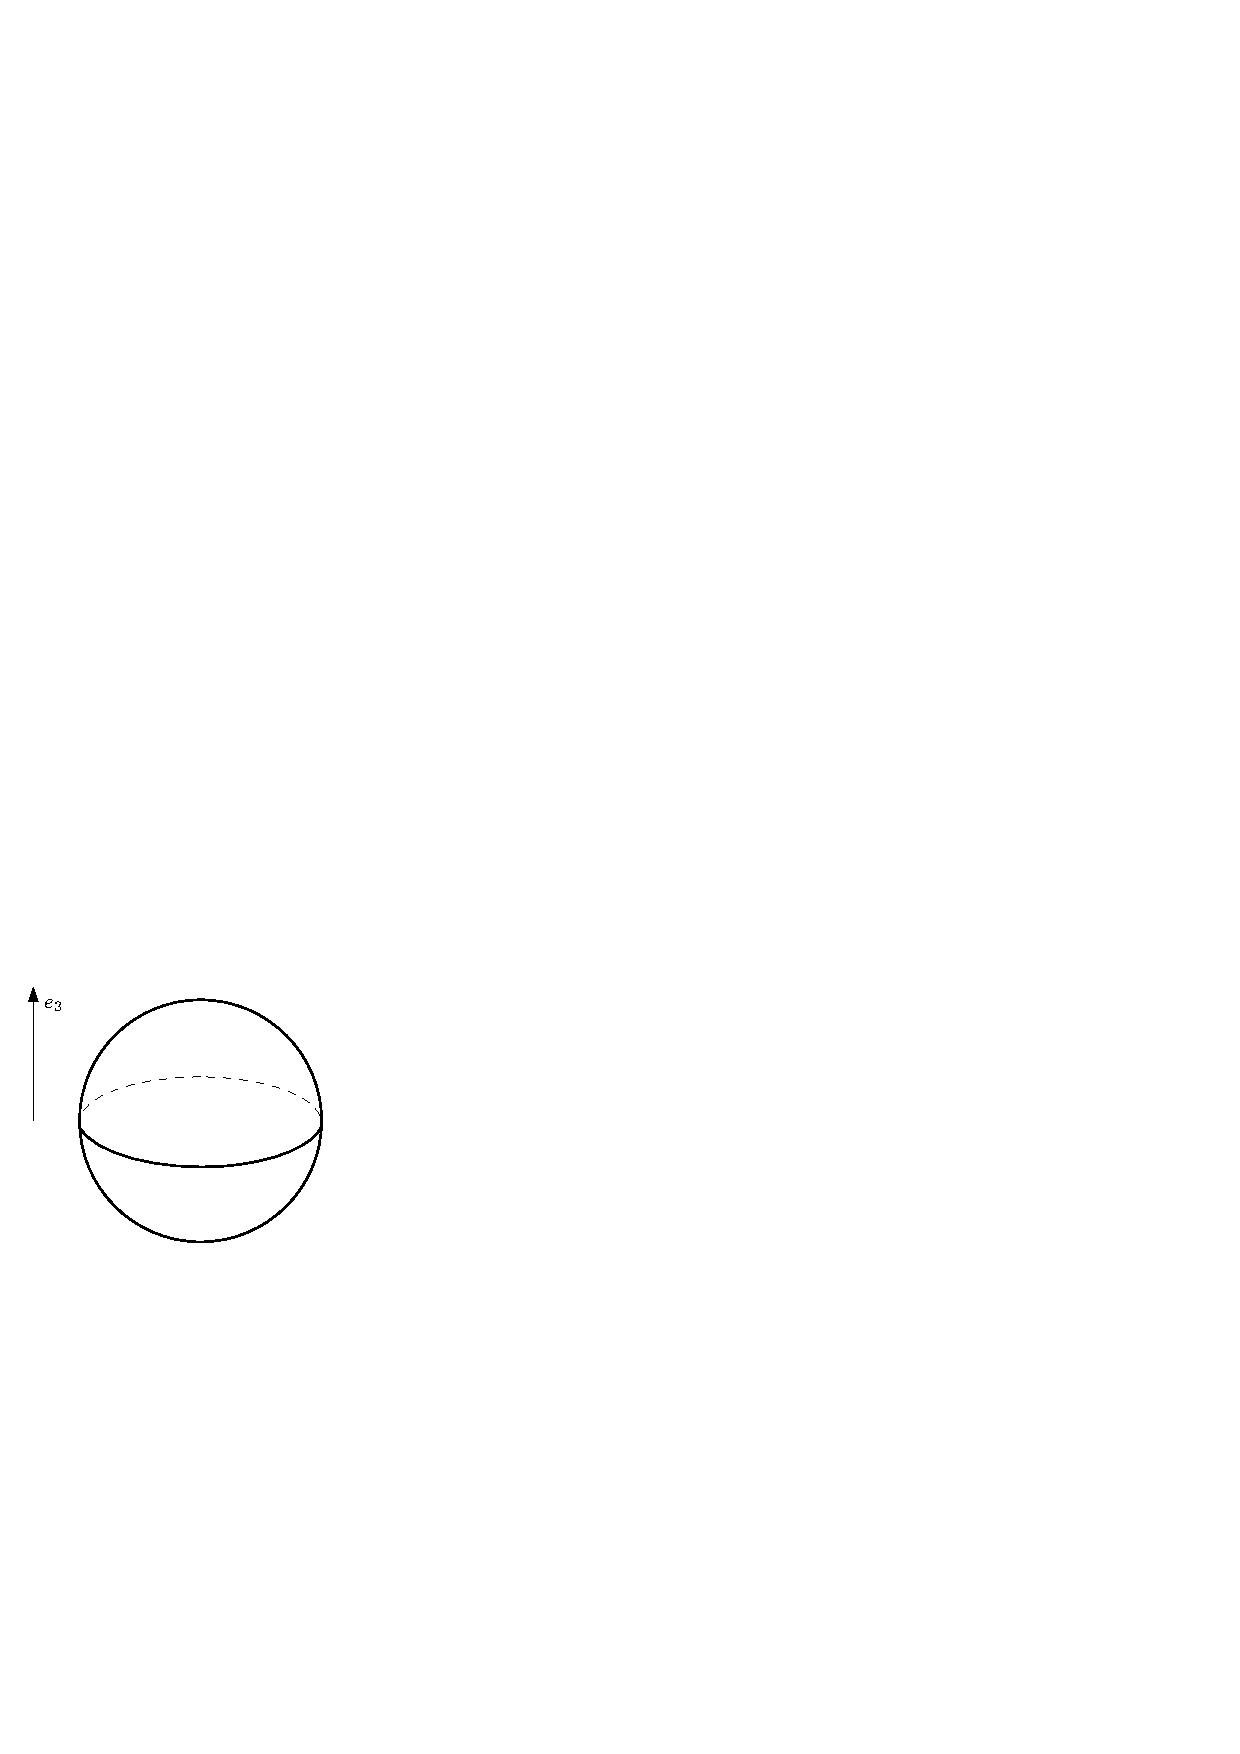
\includegraphics[scale=0.9, trim=0 0 0 0]{ball-slices}
  \caption[Slice of a ball]{The set $K_0$ where $K$ is a
    three-dimensional Euclidean ball centered at the origin. $K_0$ is
    a slice of the ball given by intersecting it with a horizontal
    plane through the origin.}
  \label{fig:ball-slices}
\end{figure}

\begin{figure}[htp]
  \centering
  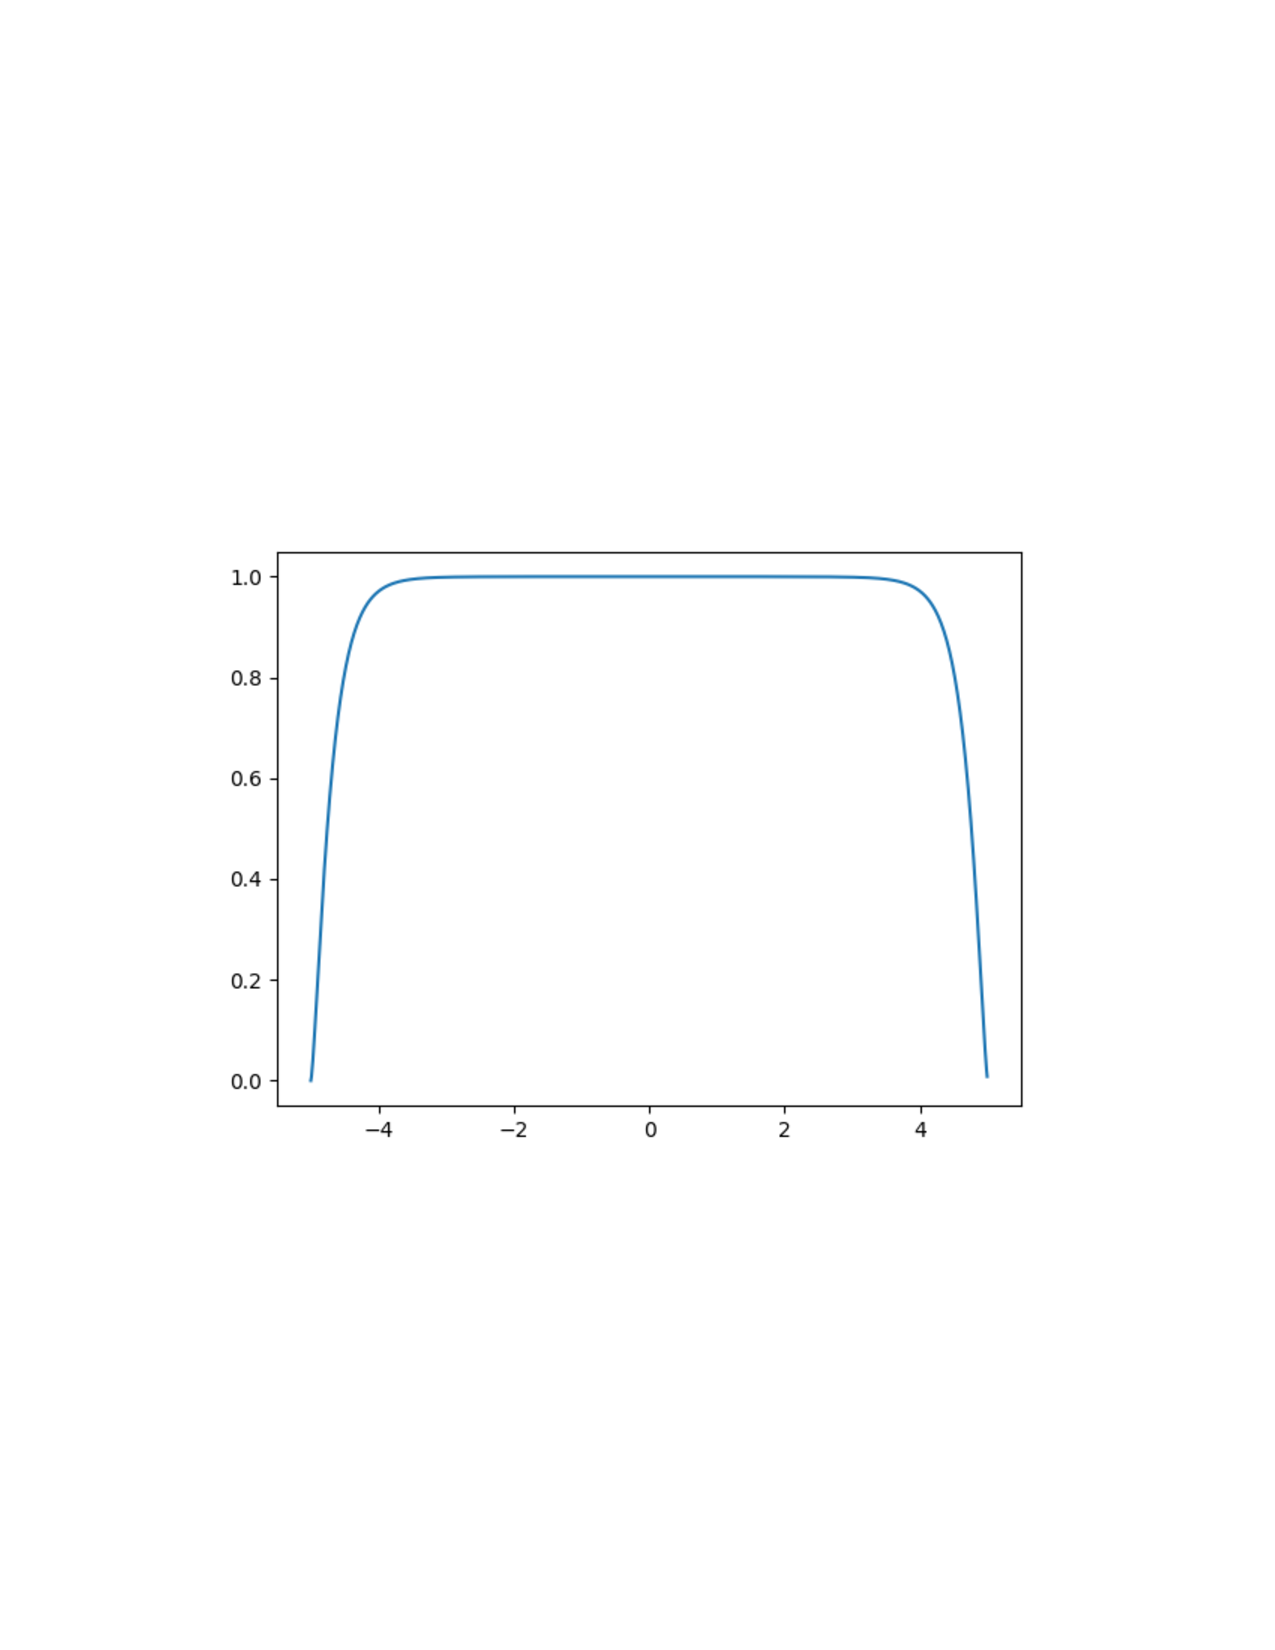
\includegraphics[scale=0.5, trim = 0 0 0 0]{ball-slices-vol3d}
  \caption[Measures of slices of a ball]{The Gaussian measure of $K_t$
    as a function of $t$, where $K$ is a three-dimensional Euclidean
    ball of radius $5$. Here $K_t$ is a two-dimensional circle of
    radius $\sqrt{25-t^2}$. Notice the measure is quasiconcave, i.e.,
    the set $\{t: \gamma^3(K_t) \ge \alpha\}$ is an interval for any
    \(\alpha\).}
  \label{fig:ball-slices-vol3d}
\end{figure}

Let \(K\subseteq \R^n\) be a closed convex
set. Lemma~\ref{lm:ch3-bm-gauss} allows us to characterize how the
Gaussian measure of sections of \(K\) changes as we slice it in a given
direction. For ease of notation, we choose the direction to be
\(e_n\), the \(n\)-th standard basis vector. This does not really cost
us any generality, since the standard Gaussian measure is invariant
under rotations. Let us then define the function
\(
  f_K(t) \eqdef \gamma^{n-1}(K_t),
\)
where \(K_t \eqdef \{y \in \R^{n-1}: (y,t) \in K\}\) is the slice of
 \(K\) consisting of points whose  \(n\)-th coordinate is equal to \(t\). See
Figures~\ref{fig:ball-slices}~and~\ref{fig:ball-slices-vol3d} for an example. Lemma~\ref{lm:ch3-bm-gauss} now tells us that \(f_K\) is
log-concave, \ie, for any \(s,t \in \R\) and any \(\lambda \in
(0,1)\),
\begin{equation}
  \label{eq:ch3-logc}
  f_K(\lambda s + (1-\lambda)t) \ge f_K(s)^\lambda f_K(t)^{1-\lambda}.
\end{equation}
Indeed, by the convexity of \(K\), \(\lambda K_s + (1-\lambda)K_t
\subseteq K_{\lambda s + (1-\lambda)t}\), and
Lemma~\ref{lm:ch3-bm-gauss} gives
\[
  f_K(\lambda s + (1-\lambda)t)
  \ge
  \gamma^{n-1}(\lambda K_s + (1-\lambda)K_t)
  \ge f_K(s)^\lambda f_K(t)^{1-\lambda}.
\]

Notice that when \(K\) is centrally symmetric, i.e.,
\(K = -K\), the function \(f_K\) is even: \(f_K(-t) = f_{-K}(t) =
f_K(t)\). Together with the log-concavity inequality
\eqref{eq:ch3-logc}, used with $\lambda \eqdef \frac12$ and $s = -t$, this means that \(f_K\) is maximized at
\(0\). Moreover, observe that $\gamma^n(K)$ is the expectation of $f_K(g)$ for a one-dimensional Gaussian $g$:
\begin{align}
\gamma^n(K) &= \frac{1}{(2\pi)^{n/2}} \int_K e^{-\|x\|_2^2/2}dx\notag\\
&= \frac{1}{(2\pi)^{n/2}} \int_{-\infty}^\infty \int_{K_t}e^{-(\|y\|_2^2 + t^2)/2}dy dt\notag\\
&= \frac{1}{\sqrt{2\pi}} \int_{-\infty}^\infty e^{-t^2/2} f_K(t)dt.\label{eq:ch3-int-slices}
\end{align}
Altogether, we have that, for centrally symmetric $K$, $f_K(0)\ge\gamma^n(K)$.

%This useful observation is recorded in the next corollary.

%\begin{corollary}\label{cor:ch3-slice-max}
%  For any centrally symmetric closed convex set \(K\) in \(\R^n\), and
%  for any hyperplane \(H\) containing \(0\), we have
%  \[
%    \gamma^H(K\cap H) := \frac{1}{(2\pi)^{(n-1)/2}}\int_{K\cap H}
%    e^{-\|x\|_2^2/2}dx \ge \gamma^n(K).
%  \]
%\end{corollary}



Equipped with the log-concavity of slice measures (inequality
\eqref{eq:ch3-logc}), we are ready to prove Sidak's lemma.

\begin{proof}[Proof of Lemma~\ref{lm:ch3-sidak}]
  We first note that the lemma is trivial for \(n=1\). In that case,
  \(K\) and \(S\) are both closed intervals symmetric around
  \(0\), and \(K \cap S\) is the smaller of the two intervals. We have
  \[
    \gamma^1(K \cap S) = \min\{\gamma^1(K),\gamma^1(S)\}
    \ge \gamma^1(K)\gamma^1(S).
  \]

  Inequality \eqref{eq:ch3-logc} and a simple computation let us
  reduce the higher dimensional case to the one dimensional one. We can  assume, by rescaling $u$, that $S = \{x \in \R^n: |\ip{u,x}| \le t\}$ and $\|u\|_2 = 1$. By
  the rotation invariance of the standard Gaussian measure, we may also
  assume that \(u = e_n\), the $n$-th standard basis vector.  Therefore,
  \(
  S = \left\{x \in \R^n: x_n \in \left[-t,t\right]\right\}.
  \)
  Note that, using \(\grv\) for a standard Gaussian random variable in \(\R^n\),
  \begin{align*}
    \gamma^n(S) = \Pr\left[|\grv(n)| \le t\right]
    = \gamma^1\left(\left[-t,t\right]\right).
  \end{align*}
  %Let \(I_K(s) \eqdef \{r\in \R: f_K(r) \ge s\}\). 
  Applying \eqref{eq:ch3-int-slices} to $K \cap S$, and noticing that $f_{K \cap S}(s)$ equals $f_K(s)$ if $s \in [-t,t]$, and $0$ otherwise, we have
  \begin{equation}\label{eq:ch3-int-sidak}
      \gamma^n(K \cap S) = \frac{1}{\sqrt{2\pi}} \int_{-t}^{t} e^{-s^2/2} f_K(s)ds.
  \end{equation}
  The right hand side is just the expected value of $f_K(g)1\{g \in [-t,t]\}$ for a standard $1$-dimensional Gaussian random variable $g$. Using integration by parts, this expectation equals
  \begin{equation} \label{eq:ch3-int-parts}
      \int_{0}^\infty \Pr[f_K(g)1\{g \in [-t,t]\} \ge r]dr
      = \int_{0}^\infty \gamma^1\left(I_K(r)\cap\left[-t,t\right]\right)dr,
  \end{equation}
  where \(I_K(r) \eqdef \{s\in \R: f_K(s) \ge r\}\). 
  By the log-concavity of \(f_K\) (inequality \eqref{eq:ch3-logc}), the set
  \(I_K(r)\) is convex, \ie, an
  interval. Moreover, \(f_K\) is clearly continuous, so \(I_K(r)\) is
  closed, and, for \(K\) symmetric around the origin, \(f_K\) is even, and \(I_K(r)\) is also
  symmetric around the origin. Thus, by the one-dimensional case of
  the lemma,
  \[
    \gamma^1\left(I_K(r)\cap \left[-t, t\right]\right)
    \ge
    \gamma^1(I_K(r)) \gamma^1\left(\left[-t,t\right]\right)
    = \gamma^1(I_K(r)) \gamma^n(S).
  \]
  Plugging this inequality back into \eqref{eq:ch3-int-sidak}~and~\eqref{eq:ch3-int-parts}% and using integration by parts again 
  gives us
  \begin{align*}
    \gamma^n(K \cap S) %&=\int_{0}^\infty \gamma^1\left(I_K(r)\cap\left[-t,t\right]\right)dr\\
    &\ge \gamma^n(S) \int_{0}^\infty \gamma^1(I_K(r))dr\\
    &= \gamma^n(S) \int_{0}^\infty \Pr[f_K(g) \ge r]dr\\
    &= \gamma^n(S) \E[f_K(g)]\\
    &= \gamma^n(S)\int_{-\infty}^\infty e^{-s^2/2}f_K(s)ds\\
    &= \gamma^n(S)\gamma^n(K).
  \end{align*}
  Above, the first equality uses the definition of $I_K(r)$, the second uses integration by parts again, with $g$ a standard 1-dimensional Gaussian, and the last equality uses \eqref{eq:ch3-int-slices}.
\end{proof}

Let us now state a significant generalization
of Lemma~\ref{lm:ch3-sidak}: Royen's Gaussian correlation inequality.
\begin{theorem}\label{thm:ch3-gauss-cor}
  For any two closed convex sets \(K, L\) symmetric around the origin
  (\ie, \(K = -K\) and \(L = -L\)), we have
  \begin{equation}\label{eq:ch3-gauss-cor}
  \gamma^n(K \cap L) \ge \gamma^n(K) \gamma^n(L).
  \end{equation}
\end{theorem}
Theorem~\ref{thm:ch3-gauss-cor}, whose proof we omit, was known as the
Gaussian correlation conjecture and was open for many years until it
was proved by Royen~\cite{Royen14} (see also the
exposition~\cite{LM-royen}). We will use it next to bound the discrepancy of set systems induced by
permutations.
\section{Discrepancy of Permutations and Gaussian Correlation}\label{sect:ch3-corr}
Recall that the set system \((\SS,[n])\) induced by \(k\) permutations
\(\pi_1, \ldots, \pi_k\) of \([n]\) consists of prefix sets of the type
\(\{\pi_i(1), \ldots, \pi_i(j)\}\). In Chapter~\ref{ch:linalg} we used
the linear algebraic method to show that the discrepancy of such a set
system is bounded by \(O(k\log(n))\). While the dependence on \(n\) in
this bound is optimal for a constant \(k \ge n\), the dependence on
\(k\) can be improved using the partial coloring method. For example,
a careful application of Lemma~\ref{lm:ch3-partial} shows that there
exists a partial coloring of discrepancy \(O(\sqrt{k})\), as indicated
in the following exercise. In this exercise we use the notion of
canonical interval defined in Chapter~\ref{ch:linalg}.

\begin{exercise}\label{ex:ch3-kperms}
  Let \(\pi_1, \ldots, \pi_k\) be permutations of \([n]\). Consider
  the set system \((\TT,[n])\) consisting of the sets \(\pi_i(C)
  \eqdef \{\pi_i(j): j \in C\}\) for
  all \(i \in [k]\) and all canonical intervals \(C \in \CC\) as
  defined in Chapter~\ref{ch:linalg}. Using Lemma~\ref{lm:ch3-partial},
  show that there exists a partial coloring \(\col\in \{-1, 0,+1\}^n\)
  such that, for any \(C \in \CC_p \subseteq \CC\), \(|\col(C)| \lesssim
  \sqrt{k}\cdot\phi(p)\) and \(|\{i: \col(i) \neq 0\}| \ge
  n/10\). Here, \(\phi(p)\) should be a function on the
  positive integers, chosen so that \(\sum_{p = 0}^{\infty}\phi(p)\)
  converges to an absolute constant.

  Then, using canonical intervals (see Section~\ref{sec:ch2-tusnady}) conclude that \(\col\)
  satisfies \(|\col(\set)|\lesssim \sqrt{k}\) for all sets \(\set\) in
  the set system \(\SS\) induced by \(\pi_1, \ldots, \pi_k\).
\end{exercise}
%\sasho{Is this exercise too much?}
We now take a different approach to show the same
result. Recall that we proved Lemma~\ref{lm:ch3-partial} using Sidak's
lemma (Lemma~\ref{lm:ch3-sidak}) and Giannopoulos's partial coloring
lemma (Lemma~\ref{lm:ch3-gian}). We will replace Sidak's lemma with
the deeper correlation inequality of Royen
(Theorem~\ref{thm:ch3-gauss-cor}), which will allow us to make the
calculations in the proof significantly simpler.

To apply Lemma~\ref{lm:ch3-gian} to the 
bound the discrepancy of a set system \((\SS,[n])\) induced by
\(k\) permutations \(\pi_1, \ldots, \pi_k\) on \([n]\), we need to
estimate the Gaussian measure of $tK$, where $K$ is the symmetric convex set
\begin{equation}\label{eq:ch3-K-perms}
K :=\left\{\col \in \R^n: \max_{\set \in \SS} |\col(\set)| \le 1\right\}.
\end{equation}
Instead of writing \(K\) as the
intersection of \(|\SS|\) many slabs, one for each set \(\set \in
\SS\), we define \(k\) convex sets \(K_1, \ldots, K_k\) where
\begin{equation}\label{eq:ch3-Ki}
K_i :=\left\{\col \in \R^n: \max_{\set \in \SS_i} |\col(\set)| \le 1\right\}
\end{equation}
and \(\SS_i\) consists of all prefix sets of the form \(\{\pi_i(1),
\ldots, \pi_i(j)\}\) for one fixed permutation \(\pi_i\). Clearly, \(K
= K_1 \cap \ldots \cap K_k\). 

We will show that, for some \(t \lesssim
\sqrt{k}\), \(\gamma^n(tK_i) \ge 2^{-n/(4k)}\), and then \(\gamma^n(tK) \ge
2^{-n/4}\) follows from Theorem~\ref{thm:ch3-gauss-cor}.
Notice that $\gamma^n(tK_i)$ is simply
\[
  \Pr[\max_{j = 1}^n\left|g(\pi_i(1)) + \ldots +
    g(\pi_i(j))\right| \le t],
\]
for a standard Gaussian
 vector \(\grv \in \R^n\). 
 
 Since the distribution of \(g\) is
invariant under permuting coordinates, this is equivalent to
estimating
\[
  \Pr\left[\max_{j = 1}^n\left|\grv(1) + \ldots + \grv(j))\right| \le t\right].
\]
That is, the probability that an \(n\) step
random walk on the real line with standard Gaussian steps starting at
\(0\) stays between \(-t\) and \(+t\). This is a question we
can answer using standard results from probability theory. It is
convenient to work instead with a continuous random process, in
particular, Brownian motion. Standard Brownian motion is a random
process $\{B(s): s \ge 0\}$ such that
\begin{itemize}
\item $B(0) = 0$ with probability 1;
\item for all integers $k > 1$, and all times $0 \le s_1 \le \ldots
  \le s_m$, the increments $B(s_1)-B(0)$, $B(s_2) - B(s_{1})$, $\ldots$, $B(s_m) -
  B(s_{m-1})$ are jointly independent;
\item for all $s \ge 0$ and $\Delta\ge 0$, $B(s+\Delta) - B(s)$ is
  distributed as a Gaussian with mean $0$ and variance $\Delta$;
\item $B(s)$ is almost surely continuous as a function of $s$.
\end{itemize}
For a proof of the non-trivial fact that Brownian motion exists,
see~\cite{PeresMorters}. It is well-known that Brownian motion
satisfies the following small ball inequality: for all $t > 0$, 
\begin{equation}
  \label{eq:ch3-bm-small}
  \Pr\Big[\sup_{s \in [0,1]} |B(s)| \le t\Big] \gtrsim \exp(-\pi^2/8t^2).
\end{equation}
For a derivation, see,
\eg, equation (7.1) of Ledoux's lecture notes~\cite{Ledoux96}. We
claim that \eqref{eq:ch3-bm-small} implies a similar bound for
$\max_{j = 1}^n\left|\grv(1) + \ldots + \grv(j)\right|$.
To see this, note that the vectors $(\grv(1), \ldots, \grv(n))$ and
$\sqrt{n}(B(1/n) - B(0),\ldots, B(1) - B((n-1)/n))$ are identically
distributed. Therefore,
\begin{align}
  \Pr\left[\max_{j = 1}^n\left|\grv(1) + \cdots + \grv(j)\right| \le t\right]
  &=
    \Pr\left[\max_{j = 1}^n\left|B(j/n)\right| \le t/\sqrt{n}\right]\notag\\
  &\ge
    \Pr\Big[\sup_{s \in [0,1]} |B(s)| \le t/\sqrt{n}\Big]\notag\\
  &\gtrsim    \exp(-\pi^2n/8t^2).\label{eq:ch3-smallball}
\end{align}

% For Brownian motion we also have the tail inequality for each $t > 0$
% \[
%   \Pr\left[\sup_{s \in [0,1]} |B(s)| \ge t\right]
%   \le 2\Pr[|B(1)| \ge t] =
%   2\left(1-\gamma^1\left(\left[-t,t\right]\right)\right),
% \]
% which follows, for example, from Theorem 2.18 in M\"{o}rters and
% Peres's book~\cite{PeresMorters}. Similarly to above, this implies
% \begin{equation}
%   \label{eq:ch3-rw-tail}
%     \Pr\left[\max_{j = 1}^n\left|\grv(1) + \ldots + \grv(j))\right|  \ge t\right]
%     \le
%     2\left(1-\gamma^1\left(\left[-\frac{t}{\sqrt{n}},\frac{t}{\sqrt{n}}\right]\right)\right).    
% \end{equation}

% To begin,
% we have the following classical result, which is useful when \(t\) is on
% the order of \(\sqrt{n}\). It follows, for example, from a stronger
% result for Brownian motion (). 

% \begin{lemma}\label{lm:ch3-rw-max}
%   Let \(\grv\) be a standard Gaussian random vector in \(\R^n\). Then,
%   \begin{align*}
%     \Pr\left[\max_{j = 1}^n\left|\grv(1) + \ldots + \grv(j))\right| \ge t\right]
%     &\le
%     2\,\Pr\left[\left|\grv(1) + \ldots + \grv(n))\right| \ge t\right]\\
%     &=
%       2\left(1-\gamma^1\left(\left[-\frac{t}{\sqrt{n}},\frac{t}{\sqrt{n}}\right]\right)\right).
%   \end{align*}
% \end{lemma}

% Lemma~\ref{lm:ch3-rw-max} gives a non-trivial bound only for values of
% \(t\) for which
% \(\gamma^1\left(\left[-\frac{t}{\sqrt{n}},\frac{t}{\sqrt{n}}\right]\right)
% > \frac12\), which only happens when \(t\gtrsim \sqrt{n}.\) We are, however,
% interested in the small ball probability setting when \(t\) is much
% smaller than \(\sqrt{n}\). Nevertheless, we can still derive the following bound using
% Lemma~\ref{lm:ch3-rw-max} by applying it to intervals of length
% roughly \(t^2\). The lemma can also be derived from lower
% bounds on the small ball probabilities for Brownian motion: see,
% \eg, equation (7.1) of Ledoux's lecture notes~\cite{Ledoux96}.

% \sasho{I lean in favour of removing this (long) proof and just leaving
%   the reference to the small ball probability result.}

% \begin{lemma}\label{lm:ch3-smallball}
%   Let \(\grv\) be a standard Gaussian random vector in \(\R^n\). There
%   exists an absolute constant \(c > 0\) such that, for any \(t \ge 2\),
%   \[
%     \Pr\left[\max_{j = 1}^n\left|\grv(1) + \ldots + \grv(j))\right|
%       \le t\right]
%     \ge c^{1+\frac{n}{t^2}}.
%   \]
% \end{lemma}
% \begin{proof}
%   We will prove the lemma for \(t\) an even integer. We can derive the
%   statement for any other \(t  \ge 2\) by replacing it by the the
%   largest even integer smaller than it. This changes the value of \(t\) by at most a
%   factor of \(2\), so the lemma still holds with a smaller \(c > 0\). 

%   Let
%   \(\ell = \frac{t^2}{4}\). Since \(t\) is an even integer, \(\ell\)
%   is an integer. Let us use the notation \(s(j) := \grv(1) + \ldots \grv(j)\) for the
%   partial sums of \(\grv\).
%   For any integer \(i \in [\lfloor n /
%   \ell\rfloor]\), we define two events:
%   \begin{itemize}
%   \item \(E_i\), the event that \(|s(j) - s((i-1)\ell)| \le
%     \frac{t}{2}\) for all \(j \in \{(i-1)\ell + 1, \ldots, i\ell\}\);
%   \item \(E'_i\), the event that \(|s(i\ell)| \le
%     \frac{t}{2}\).
%   \end{itemize}
%   Additionally, we define the event \(E_{\lceil n/\ell\rceil}\) that
%   \(|s(j) - s(\lfloor n/\ell\rfloor \ell)| \le
%     \frac{t}{2}\) for all \(j \in \{\lfloor n/\ell\rfloor \ell + 1, \ldots, n\}\).
%   By the triangle inequality, if all events \(E_1, \ldots, E_{\lceil n
%     /  \ell\rceil}\) and \(E'_1, \ldots, E'_{\lfloor n /  \ell\rfloor}\)
%   hold simultaneously, then
%   \[|s(j)| \le |s(j) - s((i-1)\ell)| +  |s((i-1)\ell)| \le t.\]
%   In the rest of the proof, we give a lower bound on
%   \(
%   \Pr[E_1, \ldots, E_{\lceil n /  \ell\rceil}, E'_1, \ldots, E'_{\lfloor n   /  \ell\rfloor}].
%   \)

%   Observe first that, since
%   \(
%   s(j) - s((i-1)\ell) = g((i-1)\ell+1) + \ldots + g(j),
%   \)
%   by Lemma~\ref{lm:ch3-rw-max} we have that
%   \[
%     \Pr[E_i] \ge
%     2\gamma^1\left(\left[-\frac{t}{2\sqrt{\ell}},\frac{t}{\sqrt{\ell}}\right]\right)
%     - 1
%     = 2\gamma^1([-1,1])-1.
%   \]
%   Moreover, the events \(E_1, \ldots, E_{\lceil n
%     /  \ell\rceil}\) are independent, so have
%   \begin{equation}
%     \label{eq:ch3-Ei}
%     \Pr[E_1, \ldots, E_{\lceil n /  \ell\rceil}] \ge
%     \left( 2\gamma^1([-1,1])-1\right)^{\lceil n / \ell\rceil}.
%   \end{equation}

%   Next we handle the events \(E'_1, \ldots, E'_{\lfloor n /
%     \ell\rfloor}\). They are not independent, but, since \(s(1),
%   \ldots, s(n)\) is a Markov chain, and $E'_i$ is determined by
%   \(s(i\ell)\), we have that 
%   \(
%   \Pr[E'_i| E'_{i-1}, \ldots, E'_1]
%   =   \Pr[E'_i| E'_{i-1}].
%   \)
%   This observation allows us to prove a lower bound on \(\Pr[E'_1,
%   \ldots, E'_{\lceil n /  \ell\rceil}]\) using the chain rule. 
%   Since
%   \(
%   s(i\ell) - s((i-1)\ell = g((i-1)\ell+1) + \ldots + g(i\ell),
%   \)
%   is distributed like a one dimensional Gaussian with mean \(0\) and
%   variance \(\ell\), we have that
%   \begin{align*}
%     \Pr[E'_i|E'_{i-1}, \ldots, E'_{1}]
%     &= \Pr[E'_i| E'_{i-1}] \\
%     &= \Pr\left[|s(i\ell)| \le \frac{t}{2} \Bigg| |s(i(\ell-1))|\le \frac{t}{2}\right]\\
%     &\ge \inf_{a: |a| \le \frac{t}{2}}
%     \Pr\left[| a + s(i\ell) -  s((i-1)\ell| \le \frac{t}{2}\right]\\
%     &= \inf_{a: |a| \le \frac{t}{2}}
%     \gamma^1\left(\left[-\frac{t}{2\sqrt{\ell}} - \frac{a}{\sqrt{\ell}},
%         \frac{t}{2\sqrt{\ell}} - \frac{a}{\sqrt{\ell}}
%       \right]\right)\\
%     &= \inf_{b: |b| \le 1}
%     \gamma^1\left(\left[-1 - b, 1 - b\right]\right).
%   \end{align*}
%   Notice that, for any \(|b| \le  1\), the interval \([-1-b,1-b]\)  is a convex  combination of \([-2,0]\) and \([0,2]\). 
%   Then the one dimensional special case of Lemma~\ref{lm:ch3-bm-gauss}
%   gives us that
%   \[
%     \inf_{b: |b| \le 1}
%     \gamma^1\left(\left[-1 - b, 1 - b\right]\right)
%     \ge
%     \gamma^1\left(\left[0, 2\right]\right).
%   \]
%   Plugging this back into the inequality above, we get
%   \begin{align}
%     \Pr[E'_1, \ldots, E'_{\lfloor n /  \ell\rfloor}]
%     &=
%       \Pr[E'_1] \Pr[E'_1|E'_2] \cdots \Pr[E'_{\lfloor n /
%       \ell\rfloor}|E'_{\lfloor n /  \ell\rfloor-1}, \ldots, E'_1]\notag\\
%     &=
%       \Pr[E'_1] \Pr[E'_1|E'_2] \cdots \Pr[E'_{\lfloor n /
%       \ell\rfloor}|E'_{\lfloor n /  \ell\rfloor-1}]\notag\\
%     &\ge \gamma^1\left(\left[0, 2\right]\right)^{\lfloor n / \ell\rfloor}.   \label{eq:ch3-Eprimei}
%   \end{align}

%   It remains to combine the two lower bounds \eqref{eq:ch3-Ei} and
%   \eqref{eq:ch3-Eprimei}. Here we use the correlation inequality
%   Theorem~\ref{thm:ch3-gauss-cor}.
%   \cut{Let, for \(i \in [\lfloor n/\ell
%   \rfloor]\), \(L_i\) and \(L'_i\) be the convex sets
%   \begin{multline*}
%     L_i \eqdef \Bigg\{x \in \R^n: |x((i-1)\ell+1) + \ldots + x(j))| \le
%                                                               \frac{t}{2}\\
%                                                               \forall j \in \{(i-1)\ell + 1, \ldots, i\ell\}\Bigg\},
%   \end{multline*}
%   and
%   \[
%     L'_i \eqdef \left\{x \in \R^n: |x(1) + \ldots + x(i\ell)| \le  \frac{t}{2}\right\}.
%   \]
%   Similarly, let
%   \begin{multline*}
%     L_{\lceil n/\ell\rceil} \eqdef \Bigg\{x \in \R^n: |x(\lfloor n/\ell\rfloor\ell+1) + \ldots + x(j))| \le
%                                                               \frac{t}{2}\\
%                                                               \forall j \in \{\lfloor n/\ell\rfloor\ell+1, \ldots, n\}\Bigg\}.
%   \end{multline*}}                                                     
%   Observe that the set of values of \(\grv\) for which the event \(E_i\)
%   holds is an intersection of symmetric slabs, and the set of values
%   for which \(E'_i\) holds is a symmetric slab. We can, therefore, define
%   symmetric convex bodies \(L_1 \cap \ldots \cap L_{\lceil n /
%     \ell\rceil}\) and \(L'_1 \cap \ldots \cap L'_{\lfloor n   /
%     \ell\rfloor}\) such that \(E_i\) is the event \(\grv \in L_i\) and \(E'_i\) is the event
%   \(\grv \in L'_i\). (We leave an explicit description of \(L_i\) and
%   \(L'_i\) as an easy exercise.) By Theorem~\ref{thm:ch3-gauss-cor}, and
%   the inequalities \eqref{eq:ch3-Ei} and \eqref{eq:ch3-Eprimei}, we have
%   \begin{align*}
%     \Pr[E_1, \ldots, E_{\lceil n /  \ell\rceil}, &E'_1, \ldots,   E'_{\lfloor n   /  \ell\rfloor}]\\
%     &=
%       \gamma^n(L_1 \cap \ldots \cap L_{\lceil n /  \ell\rceil} \cap L'_1 \cap \ldots \cap L'_{\lfloor n   /  \ell\rfloor})\\
%     &\ge
%       \gamma^n(L_1 \cap \ldots \cap L_{\lceil n /  \ell\rceil})\gamma^n(L'_1 \cap \ldots \cap L'_{\lfloor n   /  \ell\rfloor})\\
%     &=     \Pr[E_1, \ldots, E_{\lceil n /  \ell\rceil}]\Pr[E'_1,  \ldots,   E'_{\lfloor n   /  \ell\rfloor}]\\
%     &\ge
%       \left( 2\gamma^1([-1,1])-1\right)^{\lceil n /
%       \ell\rceil}\gamma^1\left(\left[0, 2\right]\right)^{\lfloor n / \ell\rfloor}\\
%     &\ge
%     \left((2\gamma^1([-1,1])-1)\gamma^1([0,2])\right)^{1+\frac{4n}{t^2}}.
%   \end{align*}
%   A numerical calculation shows that
%   \[(2\gamma^1([-1,1])-1)\gamma^1([0,2]) > 0.17 > 0.\] This completes
%   the proof. 
% \end{proof}

We can now prove the existence of a partial
coloring of discrepancy \(O(\sqrt{k})\) for any set system induced by
\(k\) permutations.

\begin{lemma}\label{lm:ch3-perms-partial}
  For any set system \((\SS,[n])\)
  induced by \(k\geq 1\) permutations of \([n]\), there exists a partial
  coloring \(\col \in \{-1, 0,+1\}^n\) such that for every
  \(\set \in \SS\), \(|\col(S)| \lesssim \sqrt{k}\), and
  \(|\{i: \col(i) \neq 0\}| \ge n/10\).
\end{lemma}
\begin{proof}
  As discussed above, it is enough to show that, for each
  \(i \in [k]\), \(\gamma^n(tK_i) \ge 2^{-n/4k}\) for some
  \(t \lesssim \sqrt{k}\). Let us first handle the case $n \ge Ck$ for
  a large enough constant $C>0$. By \eqref{eq:ch3-smallball}, we
  have
  \[
    \gamma^n(tK_i) =
    \Pr\left[\max_{j = 1}^n\left|\grv(1) + \ldots +  \grv(j)\right|  \le t\right]
    \ge c e^{-\pi^2n/8t^2},
  \]
  for a constant \(c > 0\). If $C \ge \frac{8\ln(1/c)}{\ln(2)}$, then
  it is enough to set $t \eqdef \sqrt{\frac{\pi^2 k}{\ln(2)}} \lesssim
  \sqrt{k}$ for the right hand side to be at least
  $2^{-n/4k}$.

  The proof in the case $n \le Ck$ is analogous, but, instead of
  \eqref{eq:ch3-smallball}, we use the bound
  \begin{equation}
    \label{eq:ch3-rw-tail}
    \Pr\left[\max_{j = 1}^n\left|\grv(1) + \ldots + \grv(j)\right|  \ge t\right]
    \le
    2e^{-t^2/2n}.    
  \end{equation}
  This inequality can be derived from an analogous one for Brownian
  motion (see, e.g., Theorem 2.18 in M\"{o}rters and
  Peres's book~\cite{PeresMorters}) as we did for
  \eqref{eq:ch3-smallball}. Therefore, $\gamma^n(tK_i) \ge 1- 2
  e^{-\frac{t^2}{2n}}$ for every $i \in [k]$, and  it suffices to make sure that
  \(
  1- 2e^{-\frac{t^2}{2n}} \ge 2^{-\frac{n}{4k}}.
  \) %\nikhil{one of the $k$'s on either left or right should be removed?}
    Analogously to inequality \eqref{eq:ch3-exp-ineq}, we can argue that this inequality holds
  for some $t \lesssim \sqrt{n\log\left({Ck}/{n}\right)}$. We can
  now check that, because $n \le Ck$, the right hand side is bounded
  by $O(\sqrt{k})$.
\end{proof}

The following theorem follows from Lemma~\ref{lm:ch3-perms-partial} by
completing the partial coloring to a full coloring in the usual way. 
\begin{theorem}\label{thm:ch3-perms}
  For any integer \(k \ge 1\), and any set system \((\SS,[n])\)
  induced by \(k\) permutations of \([n]\), we have
  \(\disc(\SS) \lesssim \sqrt{k}\log(2n).\)
\end{theorem}

As mentioned in Chapter~\ref{ch:linalg}, 
the dependence on $n$ in Theorem~\ref{thm:ch3-perms} is tight for any
$k \ge 3$ \cite{beck3perm}. It is open, however, whether the bound $\sqrt{k}\log(2n)$
is asymptotically tight both in $k$ and $n$. It is consistent with current knowledge that this bound can be improved to $O(\sqrt{k} + \log n)$, for example.
Note that
Lemma~\ref{lm:ch3-perms-partial} implies that the assumptions in
Lemma~\ref{lm:ch3-gian} are not sufficient to guarantee the existence
of a full, rather than partial, coloring. If they were sufficient,
then we would be able prove a constant upper bound on the discrepancy
of any set system induced by $3$ permutations, contradicting the lower
bound of Neiman, Newman, and Nikolov~\cite{beck3perm}.

An interesting question we close with is whether other classical small
ball inequalities for Gaussian processes, as well as Royen's
correlation inequality, can be useful in proving discrepancy upper
bounds.  For example, the small ball inequality for the Brownian sheet
(see again Chapter 7 of Ledoux's notes~\cite{Ledoux96}) appears to be
related to Tusn\'ady's problem (Problem~\ref{prob:tusnady}) in $2$
dimensions. 


\section{Bibliographic Notes}

The partial coloring method was first developed by Beck, who proved
Lemma~\ref{lm:ch3-beck}~\cite{beck-roth,Beck88}. He used his method to
show that the discrepancy of arithmetic progressions restricted to
$[n]$ is bounded by $n^{1/4}$ up to a factor polynomial in
$\log(n)$. This nearly matches a lower bound of Roth~\cite{roth-ap}. 

The partial coloring method of Beck was
further refined by Spencer~\cite{spencer1985} in order to prove
Theorem~\ref{thm:ch3-spencer}. Spencer's techniques are combinatorial
and do not use the geometric ideas presented in
Section~\ref{sec:ch3-giann}. The method was further refined by
Matou\v{s}ek~\cite{Matousek-halfspaces} and Matou\v{s}ek and
Spencer~\cite{MatousekSpencer-ap}. The latter paper formulated a
general partial coloring lemma similar to
Lemma~\ref{lm:ch3-partial}. Matou\v{s}ek and Spencer proved their
partial coloring lemma using an information theoretic argument due to
Boppana, initially proposed as a simplification of Spencer's proof of
Theorem~\ref{thm:ch3-spencer}~\cite{alon2000probabilistic}. Their
paper also removed the logarithmic terms in Beck's upper bound for the
discrepancy of arithmetic progressions, matching Roth's lower bound
up to a universal constant. The Matou\v{s}ek and Spencer
partial coloring lemma is sometimes also known as the entropy method.

In our presentation of the partial coloring method we depart from the
combinatorial approach and instead adopt geometric techniques
developed in the study of the vector balancing problem. The geometric
approach presented here is originally due to~Gluskin~\cite{Glu89}, who independently
proved the same discrepancy upper bound as
Spencer~\cite{spencer1985}. Lemma~\ref{lm:ch3-gian} is due to
Giannopoulos~\cite{Gia93}, who strengthened and simplified Gluskin's
results. 

Theorem~\ref{thm:ch3-bf} and Exercise~\ref{ex:ch3-komlos} are due to Giannopoulos~\cite{Gia93}, who
used Lemma~\ref{lm:ch3-gian}, and a geometric estimate of the Gaussian
measure of slices of a cube, and, independently, to
Srinivasan~\cite{Srinivasan97} who used Lemma~\ref{lm:ch3-partial}. As already mentioned, a stronger upper bound of
$O(\sqrt{\log n})$ for the Koml\'os problem was given by
Banaszczyk~\cite{Bana98} using a completely different argument not
based on partial colorings. We explain Banaszczyk's argument and its
various applications in
Chapters~\ref{ch:bana-intro}~and~\ref{ch:bana-proof}.

Lemma~\ref{lm:ch3-perms-partial} and Theorem~\ref{thm:ch3-perms} are
due to unpublished work of Spencer, Srinivasan, and
Tetali~\cite{SST-perms}. Their proof used Lemma~\ref{lm:ch3-partial},
along the lines of Exercise~\ref{ex:ch3-kperms}. The proof we present
here using Royen's correlation inequality and the small ball
inequality for Brownian motion has not been published before. We note
that some proofs of the small ball inequality \eqref{eq:ch3-bm-small}
use arguments similar to Spencer, Srinivasan, and Tetali's
argument. Other proofs rely on special properties of Brownian motion,
\eg, its connection to the Dirichlet problem.


Many other applications of the partial coloring method -- to
Tusn\'ady's problem, to giving tight bounds on the discrepancy of
halfspaces and other geometric sets, and others -- are surveyed in
Matou\v{s}ek's book~\cite{matousek2010geometric}.

%%% Local Variables:
%%% mode: latex
%%% TeX-master: "book"
%%% End:
